\section{Introduction}
\label{sec:introduction}

% state the learning objective 
\par The objective of this laboratory assignment is to study a RC circuit containing 7 resistors ($R1 to R7$), 1 sinusoidal voltage source ($V_s$), two dependent sources (one current ($G_b$) and one voltage ($H_c$)) and a capacitor ($C_a$) by determining how the voltages varie with the frequencie and time. In order to do that, natural and forced responses of the nodes are going to be needed.
The scheme of the circuit we're going to analyse and the initial given data can be seen in the figure and table below.

\begin{figure}[h] \centering
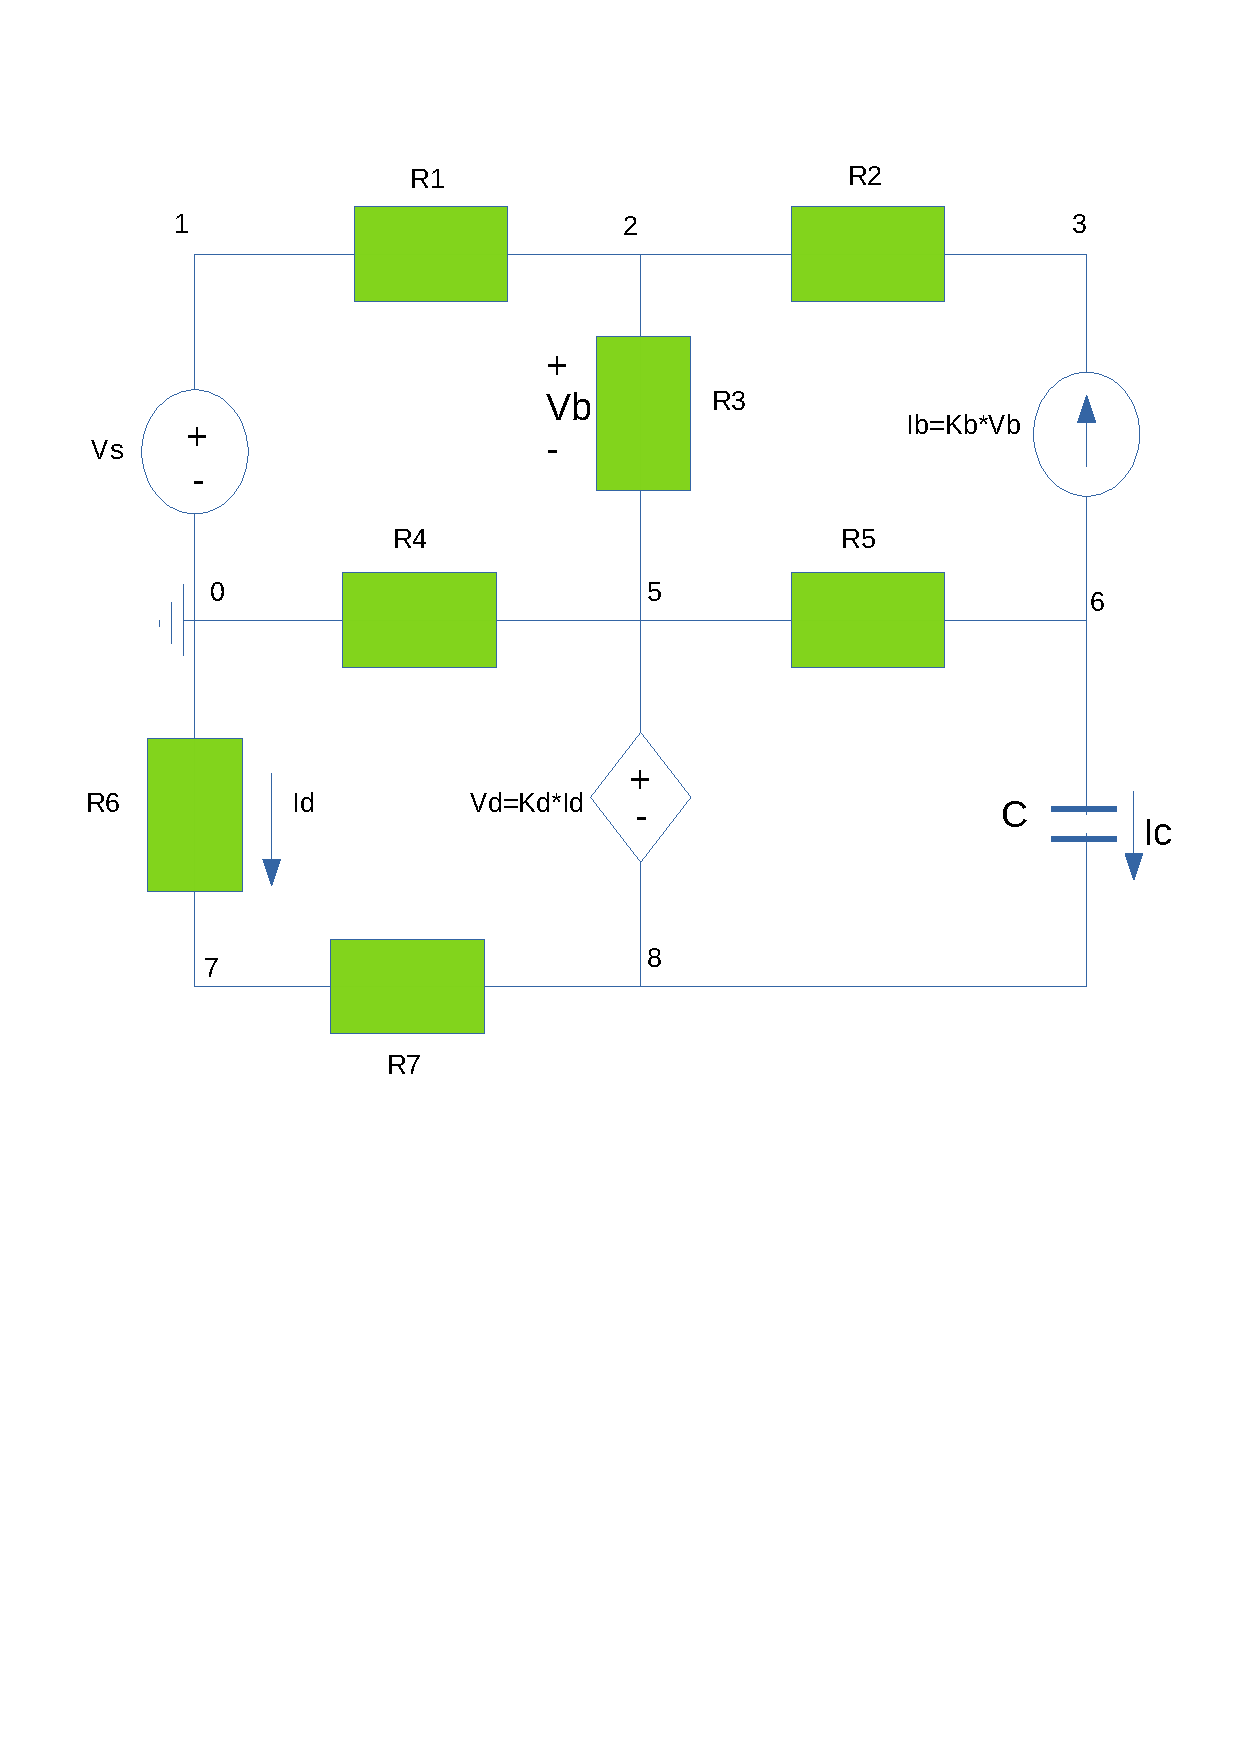
\includegraphics[width=0.6\linewidth]{Desenho_intro.odg}
\caption{Picture of the circuit in analysis}
\label{fig:V(t)}
\end{figure}

\begin{table}[H]
\centering
\begin{tabularx}{0.8\textwidth} {
  | >{\raggedright\arraybackslash}X
  | >{\raggedleft\arraybackslash}X | }
 \hline
 \caption{Initial data given by the Python script. Units in kOhm, V, F, S and A}
Amplitude1 & 1.000000e+00 V & Fase1 & 0.000000e+00 graus \\ \hline
Amplitude2 & 9.483936e-01 V & Fase2 & -1.735422e-15 graus \\ \hline
Amplitude3 & 8.415772e-01 V & Fase3 & -3.870526e-14 graus \\ \hline
Amplitude4 & 2.730068e-17 V & Fase4 & 1.800000e+02 graus \\ \hline
Amplitude5 & 9.557102e-01 V & Fase5 & 4.944819e-16 graus \\ \hline
Amplitude6 & 5.638899e-01 V & Fase6 & -1.712249e+02 graus \\ \hline
Amplitude7 & 3.731395e-01 V & Fase7 & -1.800000e+02 graus \\ \hline
Amplitude8 & 5.617171e-01 V & Fase8 & -1.800000e+02 graus \\ \hline
 data.txt
\end{tabularx}
\end{table}

\par The sinusoidal voltage source can be defined as 

\begin{equation}
  v_s(t) = V_su(-t) + sen(2pift)u(t) 
  \label{eq:vs}
\end{equation}

and,

\begin{equation}
  u(t) = 0, t<0 
  u(t) = 1, t>0
  \label{eq:u(t)}
\end{equation}

\par On the first hand, in section~\ref{ssec:Analysis}, a theoretical analysis of the circuit is
presented. Firstly, the circuit is resolver for $t<0$, then $R_eq$ is calculated by replacing the capacitor with a voltage source $V_x=V(6)-V(8)$. With it, the natural and forced responses of the circuit are calculated and then superimposed to obtain the final solution. Finally, the frequency response is also studied.

\par On the other hand, in section~\ref{ssec:Simulation} we'll simulate the same circuit in order to confirm the results seen in the previous section~\ref{ssec:Analysis}. For that similar analysis are made: for $t<0$, natural and forced responses and frequencies responses.

\par Through out the report, a comparison of the results obtain in the section~\ref{sec:simulation} and the section~\ref{sec:analysis} is made, reporting the relative errors encountered. 

\par  The conclusions of this study are outlined in section~\ref{sec:conclusion}.
